
%%%%%%%%%%%%%%%%%%%%%%%%%%%%%%%%%%%%%%%%%
% Short Sectioned Assignment
% LaTeX Template
% Version 1.0 (5/5/12)
%
% This template has been downloaded from:
% http://www.LaTeXTemplates.com
%
% Original author:
% Frits Wenneker (http://www.howtotex.com)
%
% License:
% CC BY-NC-SA 3.0 (http://creativecommons.org/licenses/by-nc-sa/3.0/)
%
%%%%%%%%%%%%%%%%%%%%%%%%%%%%%%%%%%%%%%%%%

%----------------------------------------------------------------------------------------
%	PACKAGES AND OTHER DOCUMENT CONFIGURATIONS
%----------------------------------------------------------------------------------------

\documentclass[paper=a4, fontsize=11pt]{scrartcl} % A4 paper and 11pt font size
\usepackage{epsfig}            % to insert PostScript figures
\graphicspath{
    {./eps/}
    {../MATLAB_complete/}
}
\usepackage[T1]{fontenc} % Use 8-bit encoding that has 256 glyphs
\usepackage{fourier} % Use the Adobe Utopia font for the document - comment this line to return to the LaTeX default
\usepackage[english]{babel} % English language/hyphenation
\usepackage{amsmath,amsfonts,amsthm} % Math packages
\usepackage{gensymb}
\usepackage{chemmacros}
\usepackage{graphicx,caption,subcaption}
\usepackage{sectsty} % Allows customizing section commands
\allsectionsfont{\centering \normalfont\scshape} % Make all sections centered, the default font and small caps

\usepackage{fancyhdr} % Custom headers and footers
\pagestyle{fancyplain} % Makes all pages in the document conform to the custom headers and footers
\fancyhead{} % No page header - if you want one, create it in the same way as the footers below
\fancyfoot[L]{} % Empty left footer
\fancyfoot[C]{} % Empty center footer
\fancyfoot[R]{\thepage} % Page numbering for right footer
\renewcommand{\headrulewidth}{0pt} % Remove header underlines
\renewcommand{\footrulewidth}{0pt} % Remove footer underlines
\setlength{\headheight}{13.6pt} % Customize the height of the header
\setlength{\parskip}{1em}

\numberwithin{equation}{section} % Number equations within sections (i.e. 1.1, 1.2, 2.1, 2.2 instead of 1, 2, 3, 4)
\numberwithin{figure}{section} % Number figures within sections (i.e. 1.1, 1.2, 2.1, 2.2 instead of 1, 2, 3, 4)
\numberwithin{table}{section} % Number tables within sections (i.e. 1.1, 1.2, 2.1, 2.2 instead of 1, 2, 3, 4)

\setlength\parindent{0pt} % Removes all indentation from paragraphs - comment this line for an assignment with lots of text

%general text processing
\newcommand{\supr}[1]{\ensuremath{^{#1}}}
\newcommand{\sub}[1]{\ensuremath{_{#1}}}

%----------------------------------------------------------------------------------------
%	TITLE SECTION
%----------------------------------------------------------------------------------------

\newcommand{\horrule}[1]{\rule{\linewidth}{#1}} % Create horizontal rule command with 1 argument of height

\title{	
\normalfont \normalsize 
\textsc{Universit\"{a}t Basel, Mrsic-Flogel Lab} \\ [25pt] % Your university, school and/or department name(s)
\horrule{0.5pt} \\[0.2cm] % Thin top horizontal rule
\huge Ca\supr{++} Imaging Analysis in MATLAB
\horrule{1.5pt}\\ % Thick bottom horizontal rule
}

\author{}

\date{\normalsize\today} % Today's date or a custom date

\begin{document}

\maketitle % Print the title

In this practical you will analyse 2-photon imaging data using MATLAB. This is the same approach 
neuroscientists use to analyse data in their studies. You should complete all steps by modifying the 
MATLAB functions you have been provided.


You will be supplied with with raw Ca\supr{++} imaging data from mouse V1. The mouse 
was anesthetized and was stimulated drifting black and white grating stimuli, drifting in multiple different directions. From these data
we can obtain a direction and orientation tuning curve for each cell in the field of view. Your task will be to to 
extract the raw fluorescence intensity trace from one cell, convert this to $dF/F$, and then 
determine the $dF/F$ for each stimulus in order to produce a polar plot that shows response magnitude
for different drift directions. You will then be able to select different cells and quickly pass the extracted 
response timecourses through the functions you have written to get tuning curves for several 
different cells. 


While you work through the exercise, write your responses to the questions in a word or text document. You will need to save several figures, as well as the MATLAB functions you write to solve the exercise.


Remember that typing \texttt{help function\_name} in MATLAB will give you a lot of information about how to use the function.

\subsection{Start MATLAB and download the data}
\begin{itemize}
\setlength{\parskip}{0.25em}
\item Download the data needed for this practical from \textit{http://mouse.vision/ca.zip} and unpack the zip archive. 
\item Start MATLAB.
\item Use the change directory button at the top of the screen to navigate to the 
directory containing the files you just unzipped. 
\end{itemize}

\begin{figure}
    \centering
    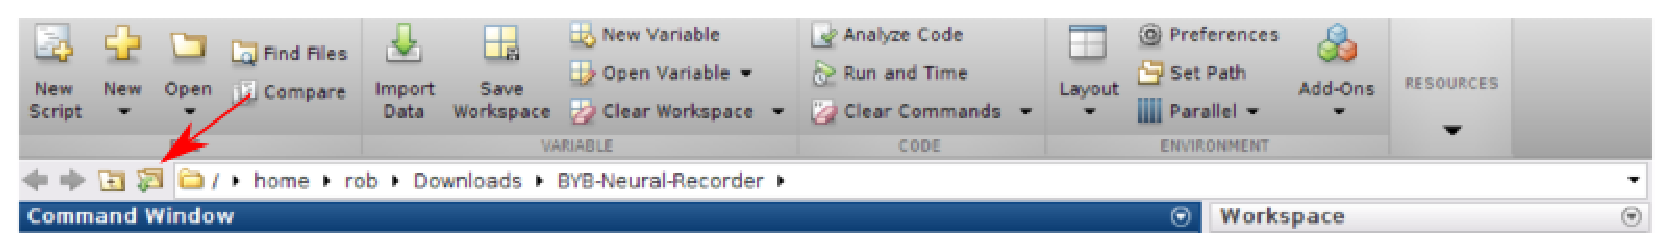
\includegraphics[width=\textwidth]{change_dir.eps}
    \caption{}
\end{figure}

\subsection{Extract response time-course from a cell}
\begin{itemize}
\setlength{\parskip}{0.25em}
\item Load the image stack called \texttt{Calcium\_imaging\_data\_int8.tif} using the \texttt{load\_stack} command.
\item Calculate the average image using the \texttt{mean} command and assign it to a variable called \texttt{meanIM}.  Plot the image using the \texttt{imagesc} command (see Figure~\ref{fig:mean_ca}). Save your image.
\item Look at the image. What does this projection tell you about the activity of different neurons?
\item Start ROI selection GUI using the \texttt{get\_roi} command.
\item Draw an ellipse around a cell to highlight it. Double-click on the ellipse, and the average time-trace of the pixels within your ROI will be returned.
\item Plot the resulting time course using \texttt{plot} (see Figure~\ref{fig:time_trace}). Save your image.
\item You will now compute the \textit{change} in fluorescence over time ($dF/F$)
	\begin{enumerate}
	\item Load the file \texttt{calc\_dF\_F.m}. This gets as input the raw trace from one cell and returns as output the $dF/F$. You will edit	the function to calculate and return the $dF/F$.
	\item Calculate $dF/F = (F-F_0)/F_0$. $F_0$ is the median of the fluorescence (F) distribution. Calculate this in the function file using the \texttt{median} command.
	\item Subtract $F_0$ value from each fluorescence ($F$) value, and then divide the resulting value by $F_0$.
	\item Run your function and plot the $dF/F$ using \texttt{plot} (see Figure~\ref{fig:time_trace_dff0}). Save your image.
	\end{enumerate}
\end{itemize}

\begin{figure}
    \centering
    
    \begin{subfigure}[b]{0.3\textwidth}
    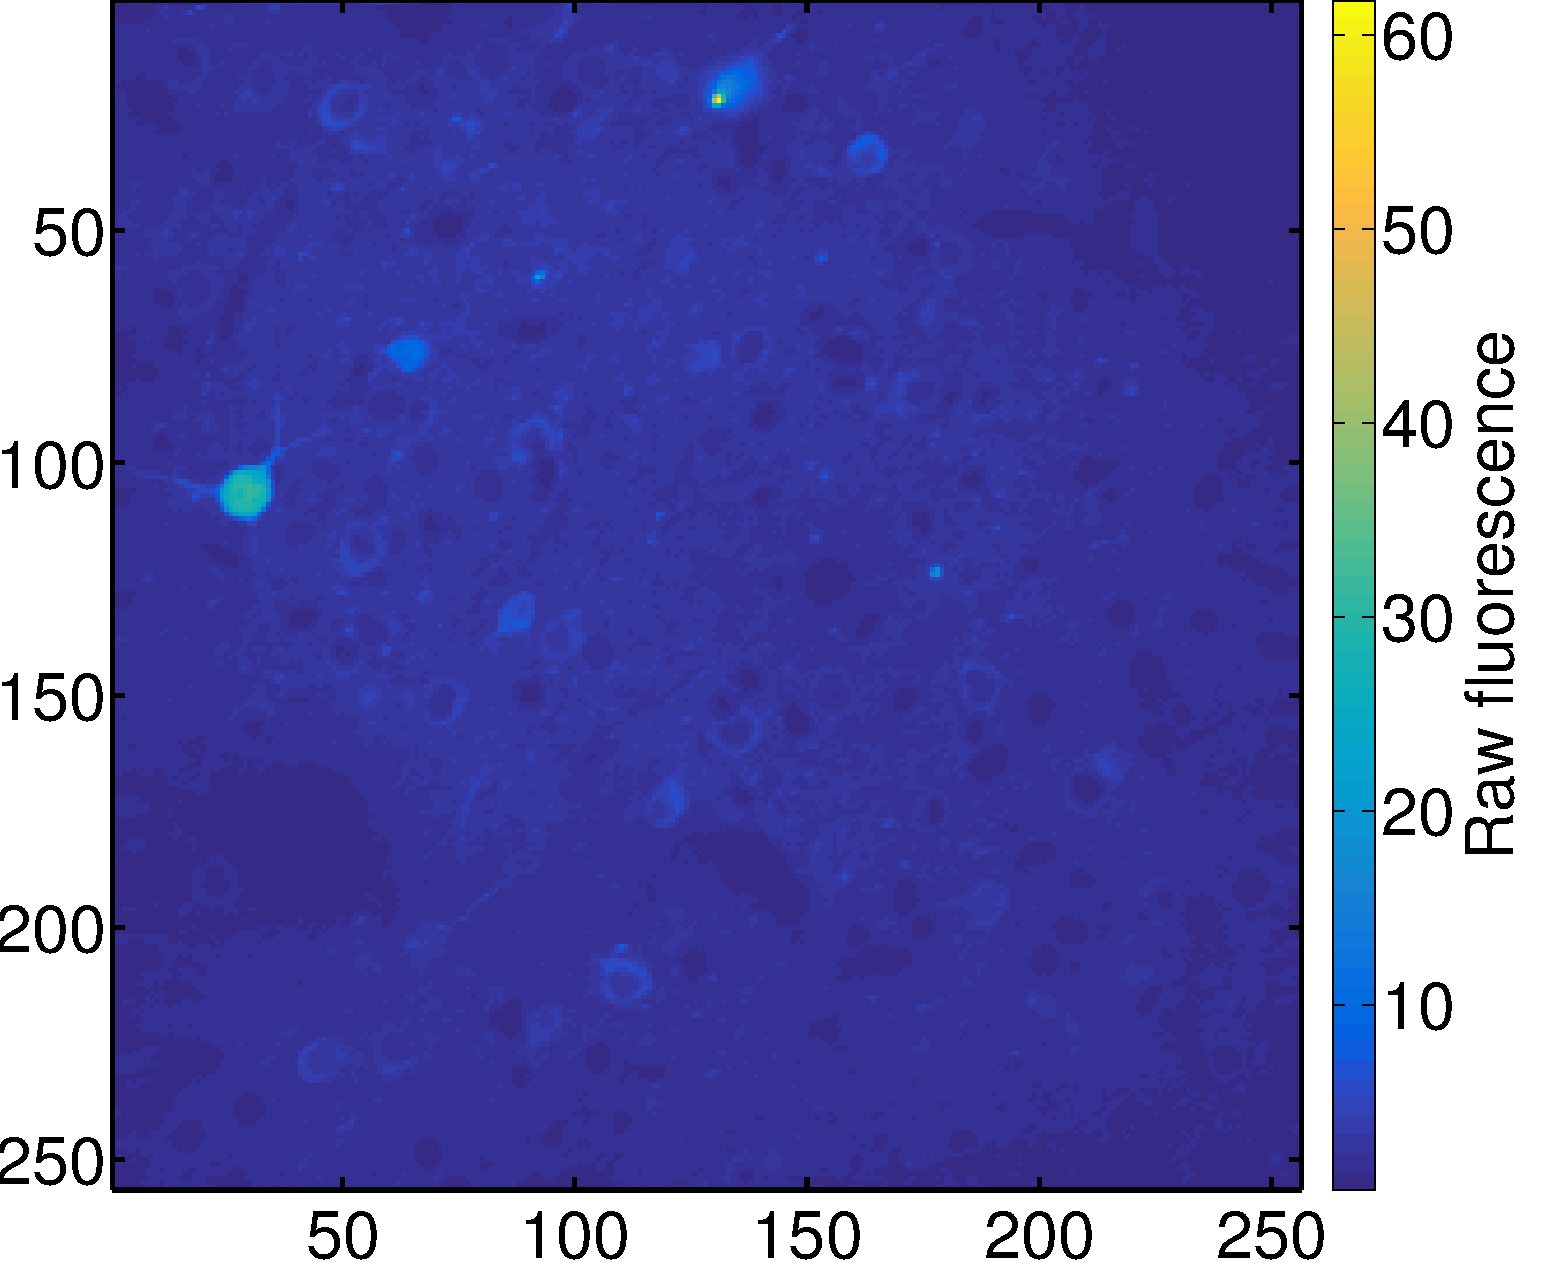
\includegraphics[width=\textwidth]{mean_image.pdf}
    \caption{Mean projection}
    \label{fig:mean_ca}
    \end{subfigure}
    \hfill
    \begin{subfigure}[b]{0.3\textwidth}
    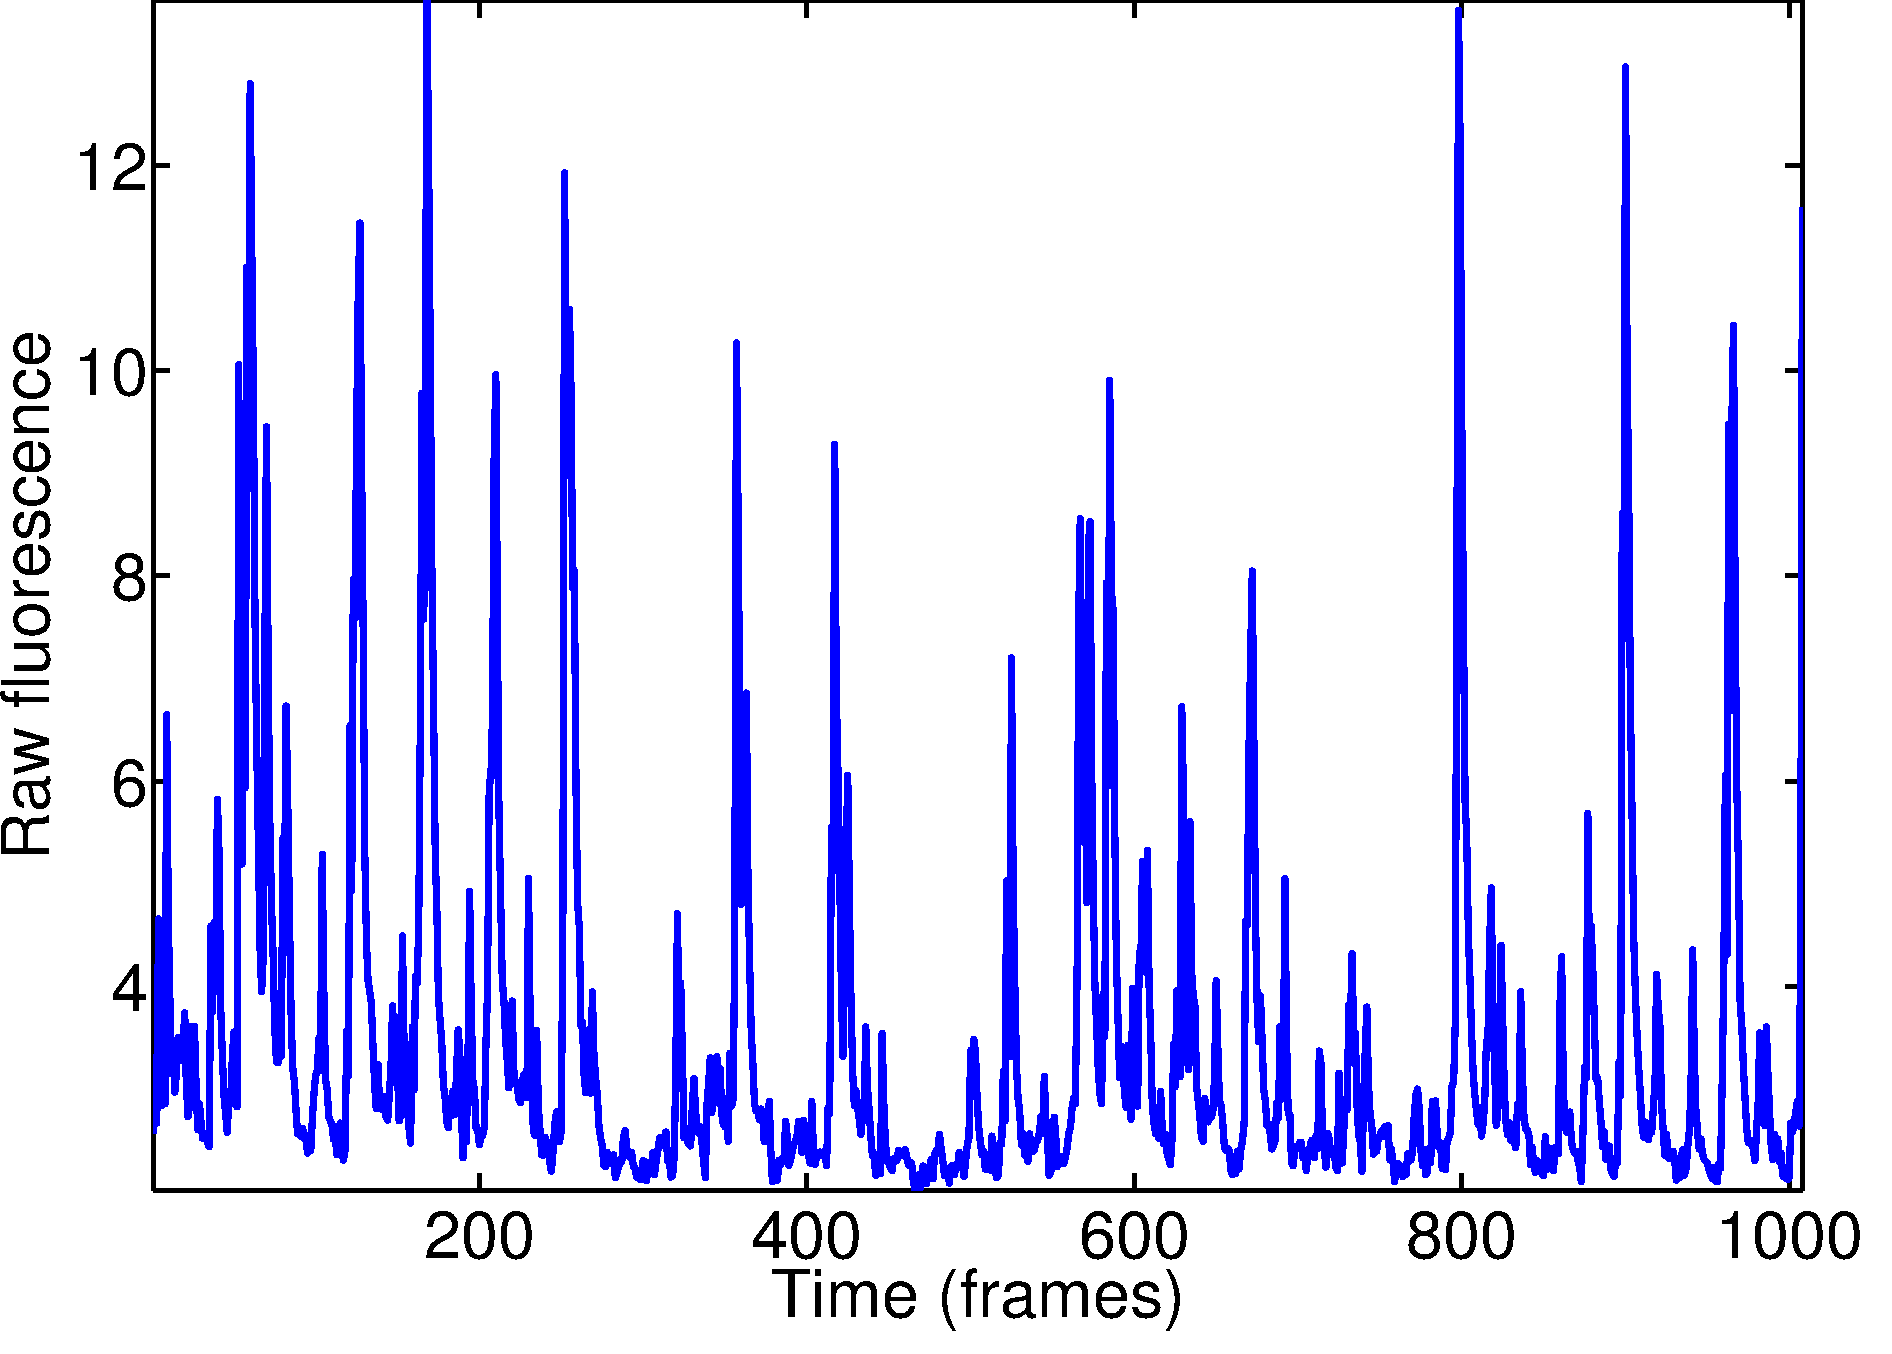
\includegraphics[width=\textwidth]{trace_raw.pdf}
    \caption{Raw fluorescence trace}
    \label{fig:time_trace}
    \end{subfigure}
    \hfill
    \begin{subfigure}[b]{0.3\textwidth}
    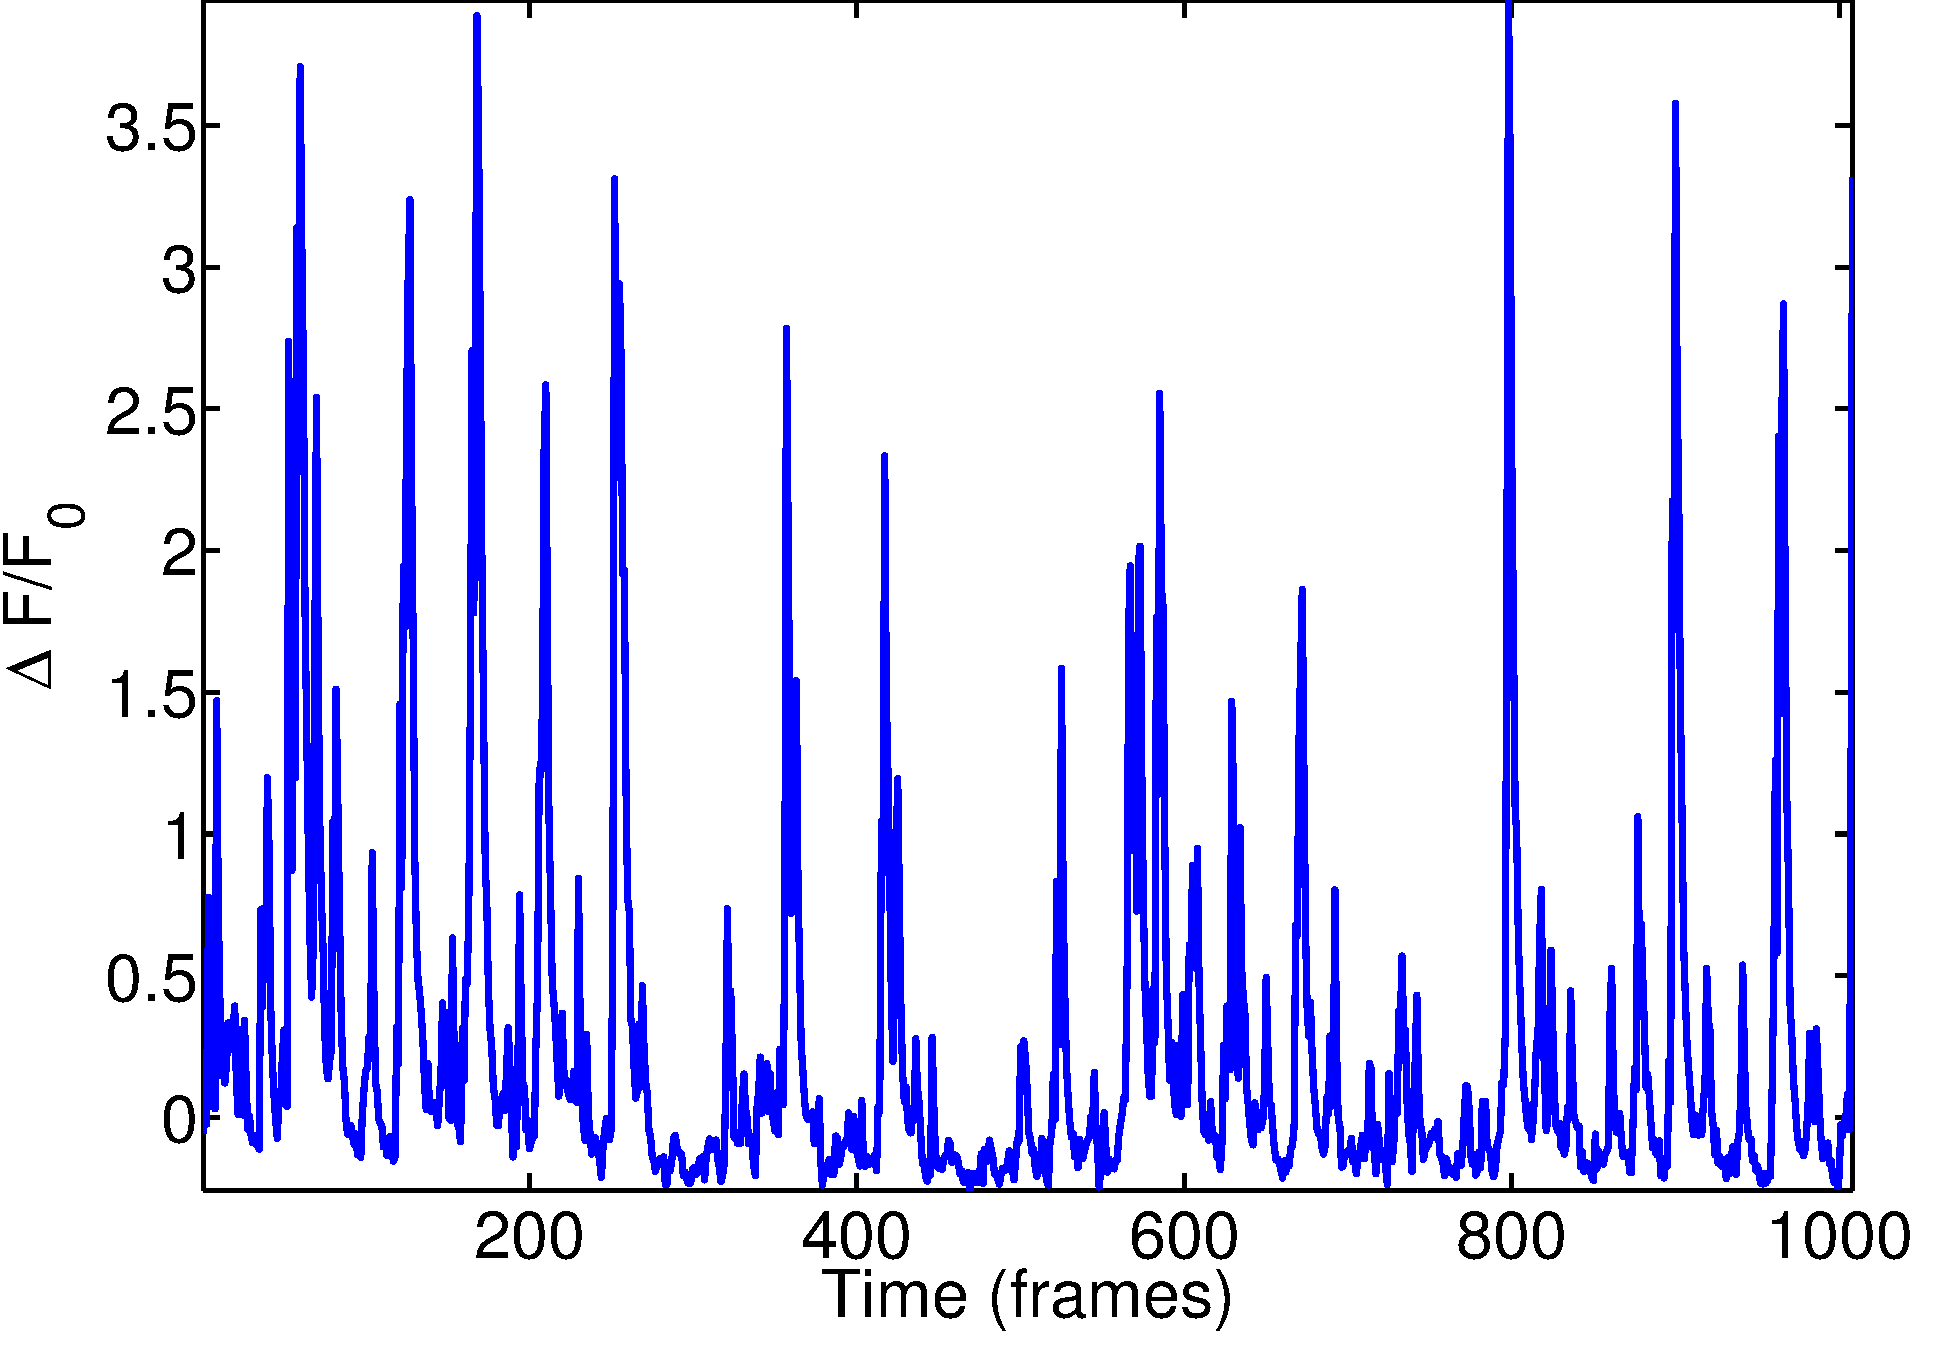
\includegraphics[width=\textwidth]{trace_delta_f_f0.pdf}
    \caption{$\Delta F/F_0$ time trace}
    \label{fig:time_trace_dff0}
    \end{subfigure}
    
    \caption{}
\end{figure}

\subsection{Understanding the stimulus presentation paradigm}
Compute the average response timecourse over multiple repetitions of the same stimulus. In this dataset, each of the 16 stimulus drift directions was presented 3 times (The drifting grating was presented for 1.5 seconds preceded by a gray screen presented for 3.5 seconds). The drift direction in degrees presented for each stimulus frame is saved in the file \texttt{ori\_stimuli.mat}.

\begin{itemize}
\setlength{\parskip}{0.25em}
\item Draw below what this stimulation paradigm looks like over time, by indicating the time in seconds for baseline and for stimulus presentation, for a single presentation of a drafting grating.\vspace{3in}
\item How many frames are in one stimulus presentation (blank+stim)? What is the imaging frame rate? Add the number of frames on your drawing above.
\item Split up the response into presentations of the same directions, over the three trials per direction. Edit file \texttt{meanTraces.m}.
\item Average the three individual trial traces for each direction and plot these average traces for each of the 16 stimulus directions on the same plot (see Figure~\ref{fig:trace_all_ori}).
\item Plot a single average trace over all stimuli. Where does the peak fall with respect to the stimulus start time? Refer to your diagram, above.
\end{itemize}

\begin{figure}
    \centering
    \begin{subfigure}[b]{0.46\textwidth}
    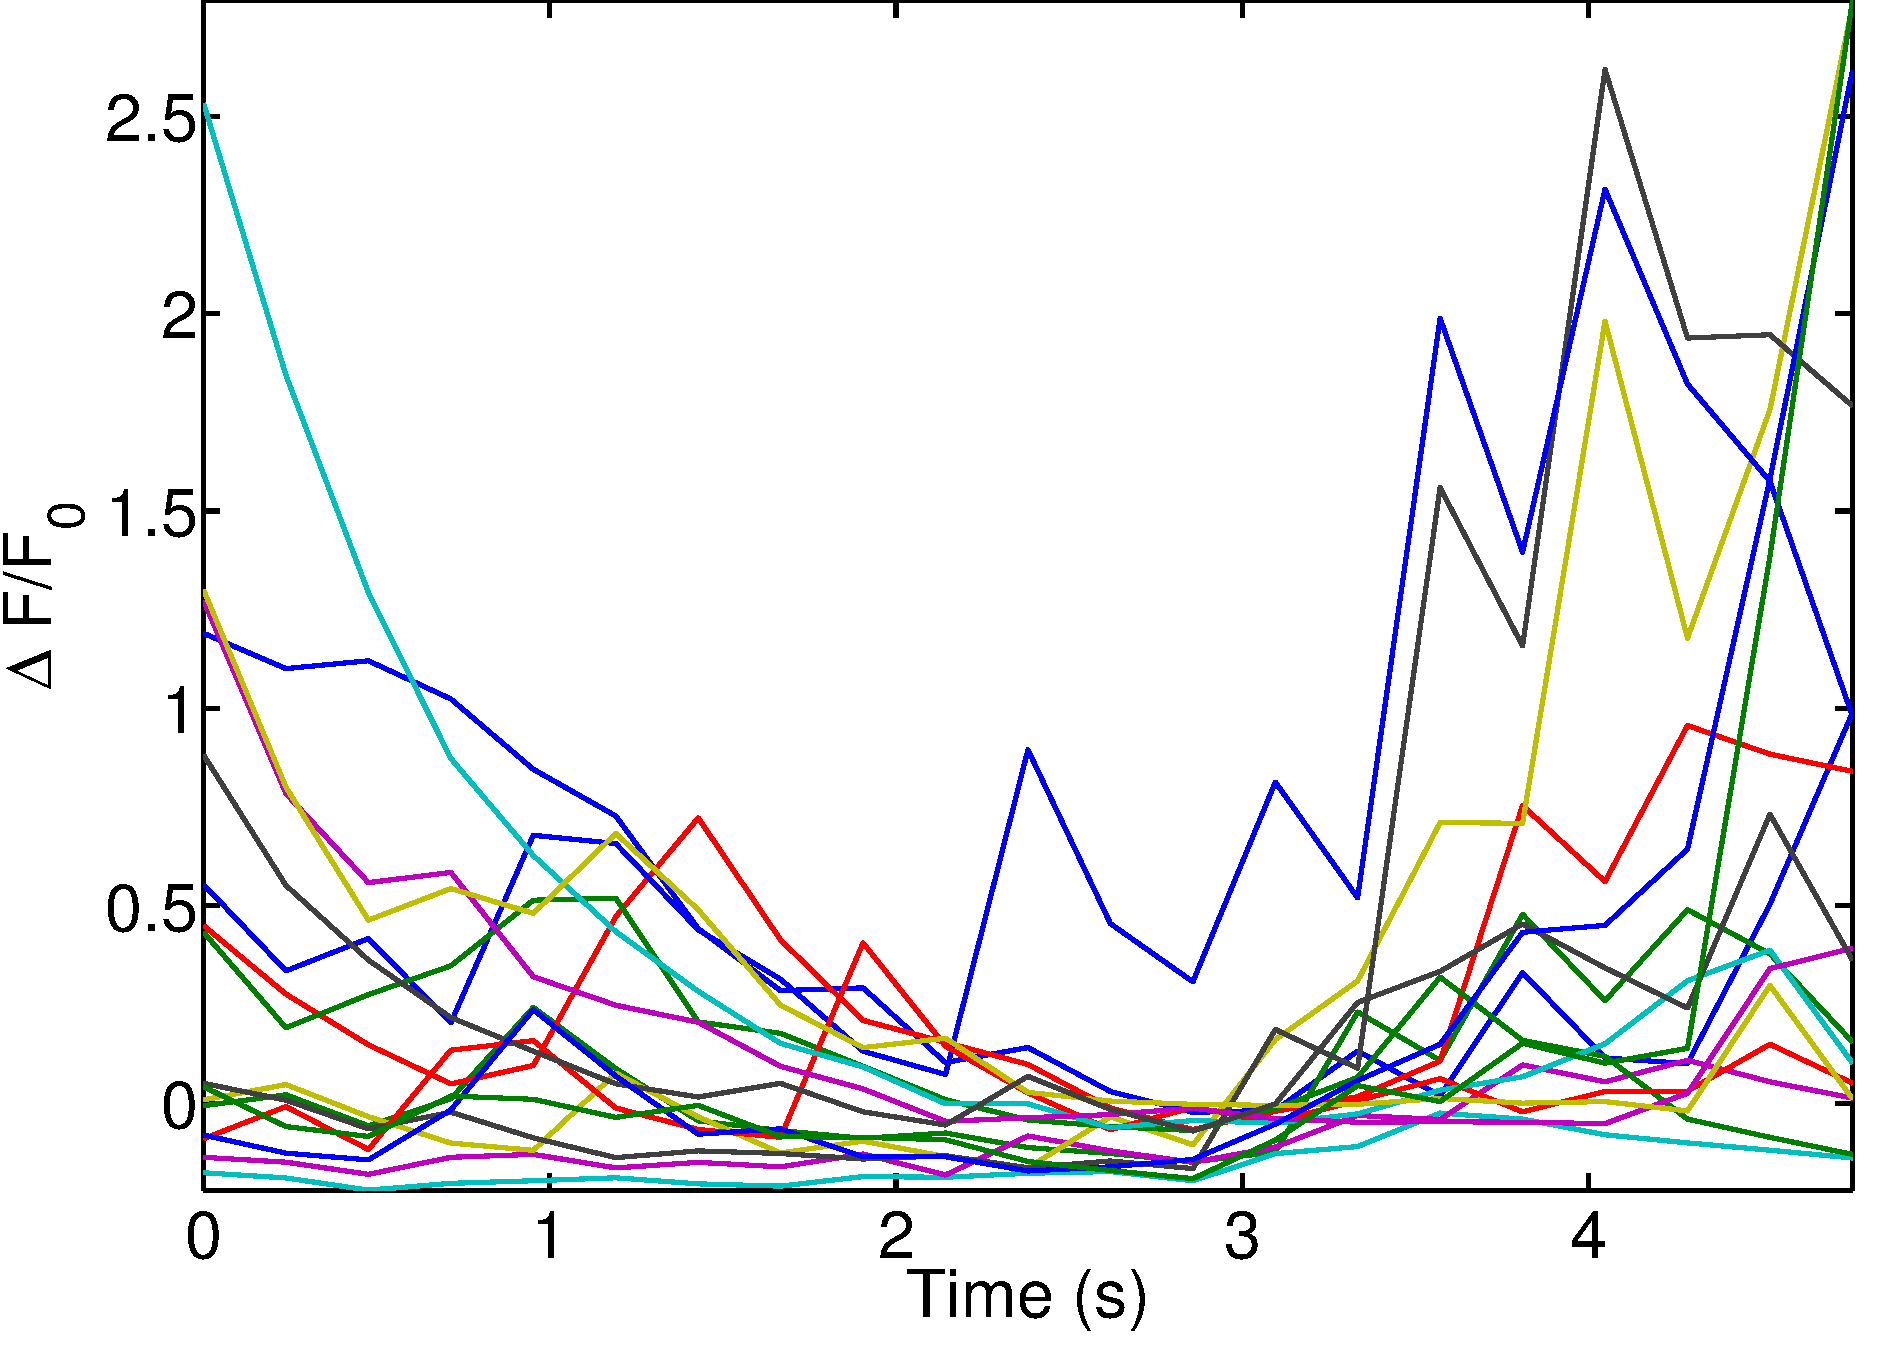
\includegraphics[width=\textwidth]{trace_dff_all_ori.pdf}    
    \caption{Average response, all orientations}
    \label{fig:trace_all_ori}
    \end{subfigure}
    \hfill
    \begin{subfigure}[b]{0.44\textwidth}
        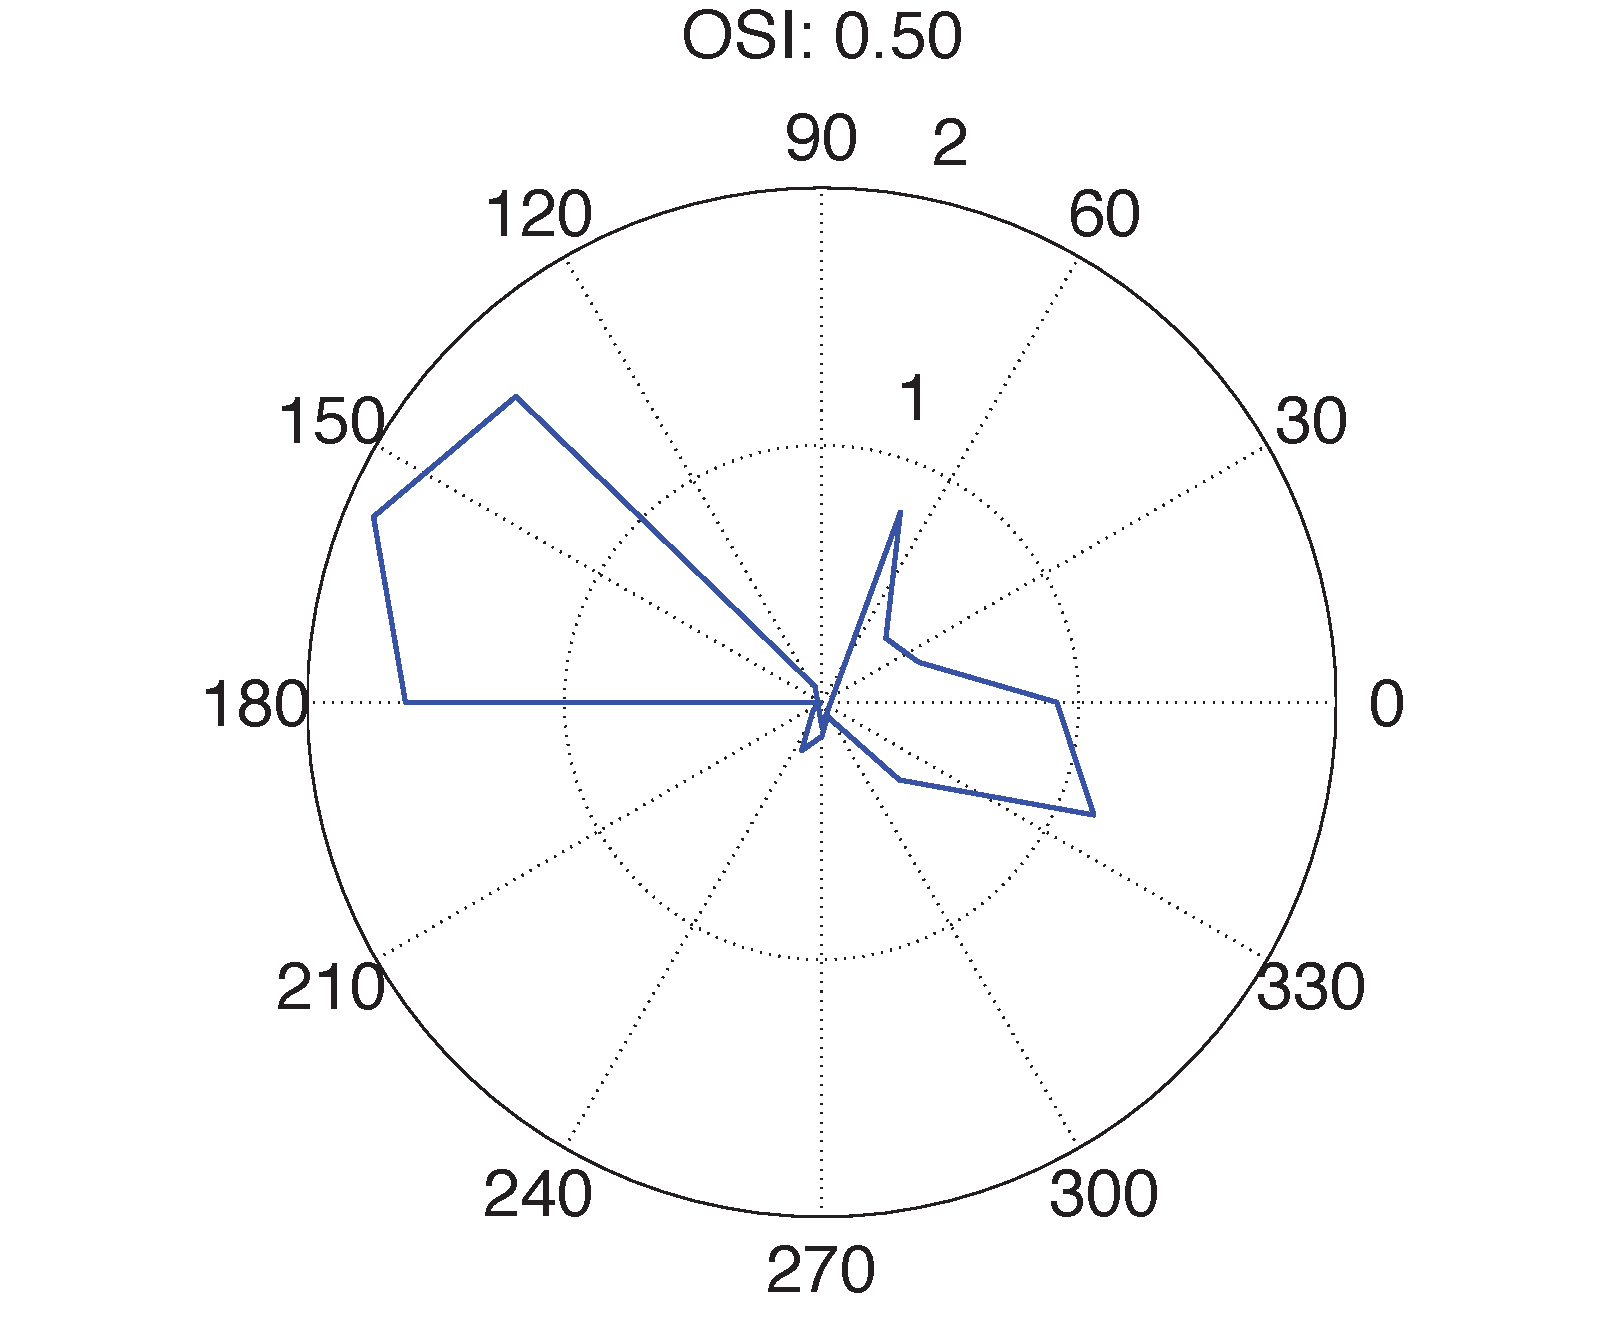
\includegraphics[width=\textwidth]{polar_ori.pdf}
        \caption{Polar plot of average response}
        \label{fig:polar_ori_plot}
    \end{subfigure}
%    \begin{subfigure}[b]{0.45\textwidth}
%    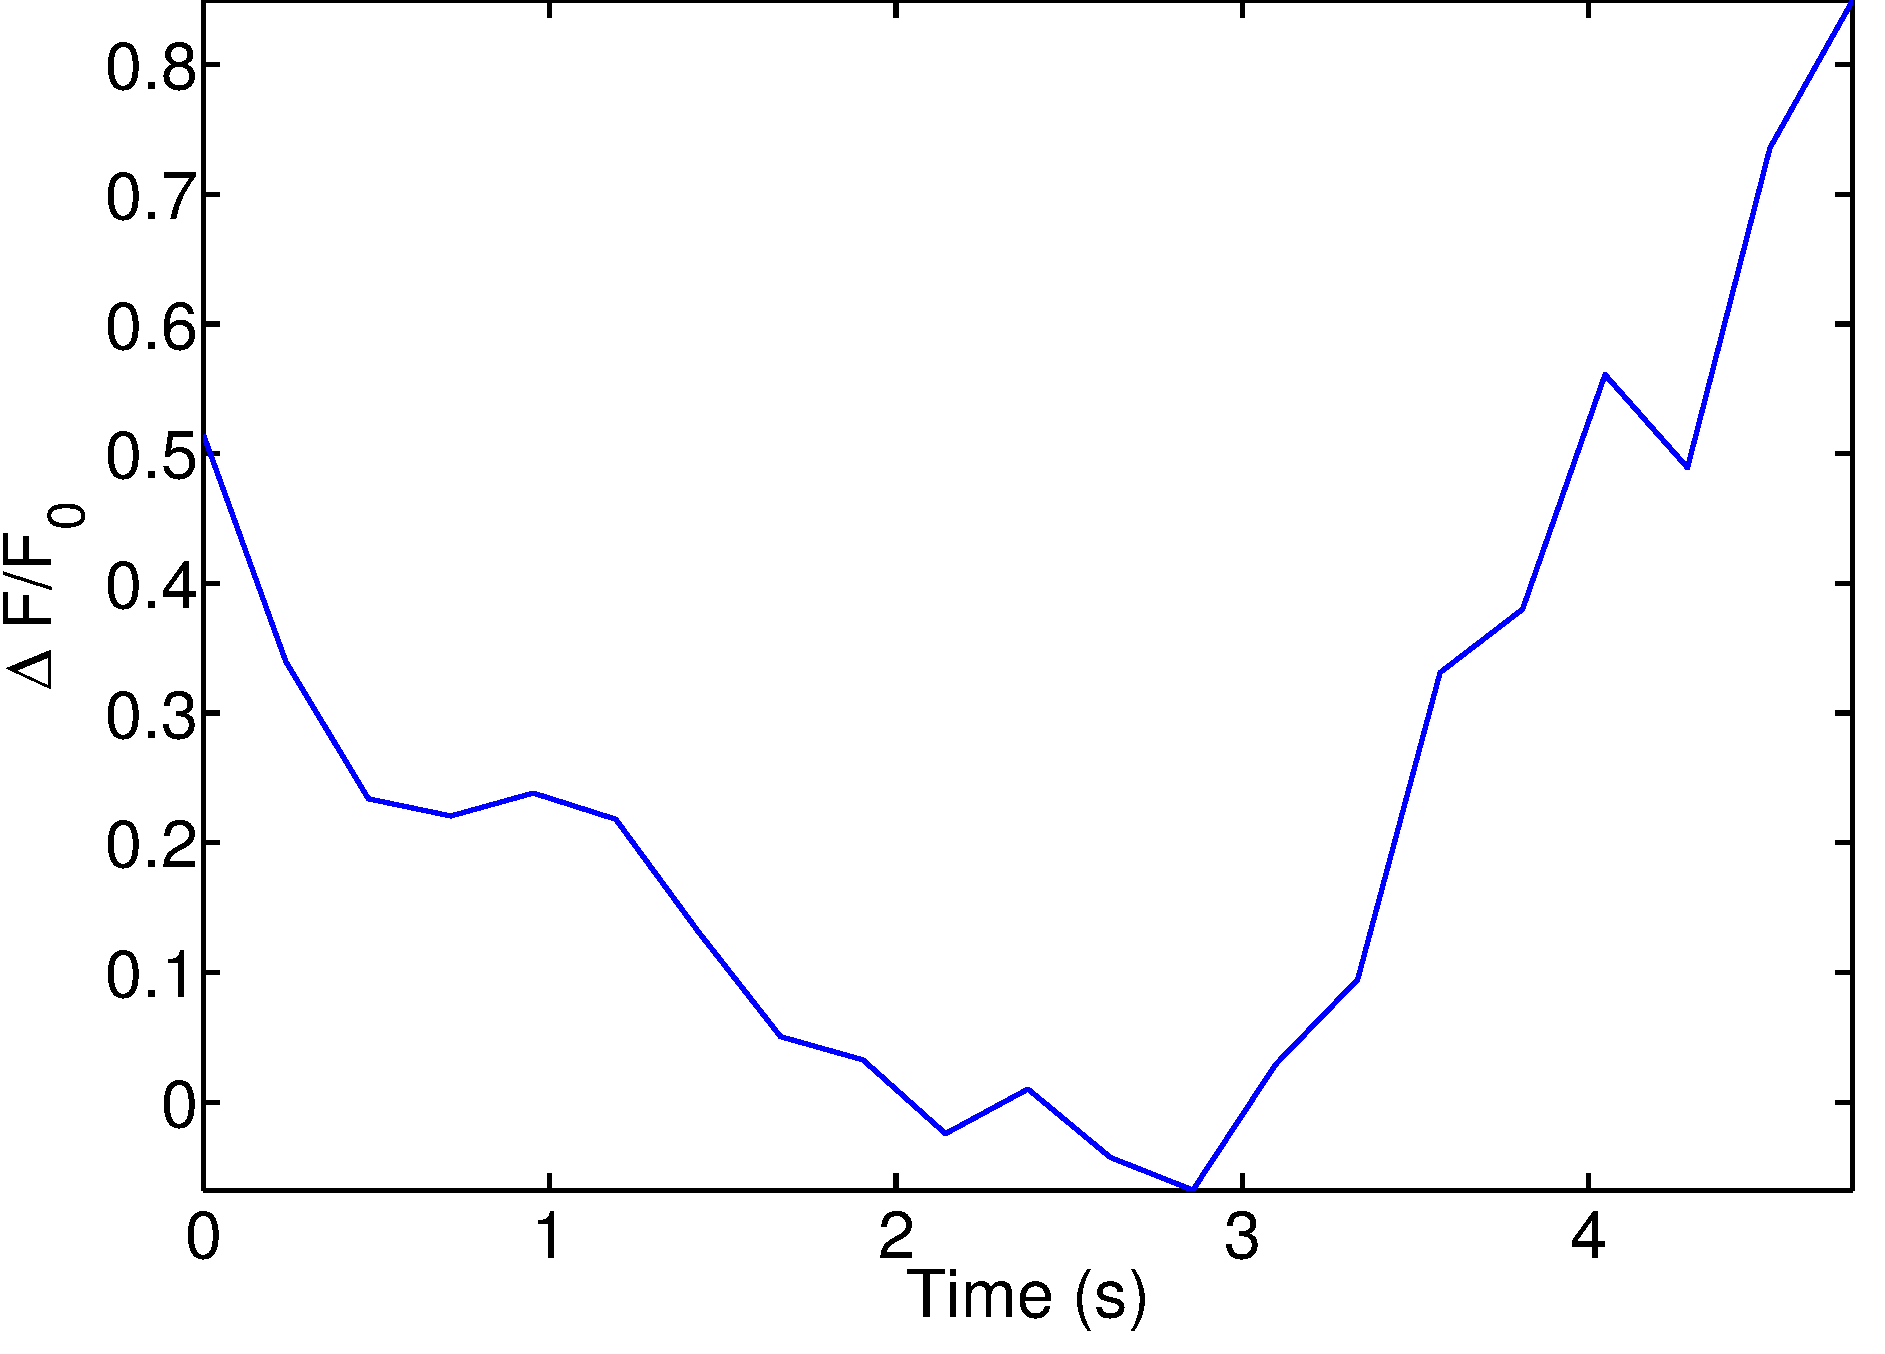
\includegraphics[width=\textwidth]{trace_dff_global_mean.pdf}    
%    \caption{Global average response}
%    \label{fig:trace_global_mean}
%    \end{subfigure}
    
    \caption{}
\end{figure}

\subsection{Calculate responses to different stimuli}
You will now find the mean response to each of the 16 stimulus orientations. Edit the file \texttt{makePolarPlot.m}.
\begin{itemize}
\setlength{\parskip}{0.25em}
\item Choose a window of 5 time points that should contain the peak response to a stimulus, during the stimulus period. Average the 5 time points within this window, from the average timecourse of each stimulus orientation.
\item Plot the mean responses on a polar plot, which will reveal the orientation tuning of the cell, using the \texttt{polar} command (see Figure~\ref{fig:polar_ori_plot}). Why is a polar plot a better choice than a conventional x/y line or scatter plot?
\item Is your cell tuned to the drift direction of the stimulus? Is your cell tuned to the drift direction of two stimuli of the same orientation?
\item Compute the orientation selectivity index (OSI):
    \begin{enumerate}
    \item Edit the file \texttt{calc\_osi.m}
    \item Find the stimulus direction that caused the biggest response (`preferred' stimulus).
    \item Find the mean response of the preferred stimulus, and the stimulus of opposite drift direction (180 degrees away), and average the two values.
    \item Find the mean response of the two stimuli that are 90 degree away from the preferred stimulus (`orthogonal' stimuli), and average the two values.
    \item Orientation selectivity index (OSI) is calculated as \\ $OSI = {\left(preferred - orthogonal\right)} / {\left(preferred + orthogonal\right)}$
    \item Add the OSI to your polar plot, using the \texttt{title} command.
    \end{enumerate}
\end{itemize}

\subsection{Repeating for other cells}
You should now have a series of files that you can call in sequence to get a polar plot: \texttt{calc\_dF\_F.m} then \texttt{meanTraces.m} then \texttt{makePolarPlot.m} then \texttt{calc\_osi.m}. If you select a new cell, you can pass it through these functions to quickly generate a polar plot. 

\begin{itemize}
\setlength{\parskip}{0.25em}
\item Create a new function called \texttt{batch.m}. Provide as an input argument the response time course. 
\item In the function body call the functions you have made in order. Passing the correct inputs and outputs to each so that you can feed \texttt{batch.m} a response time course and get back a polar plot. 
\item Run \texttt{batch.m} for 5 different cells and save the resulting plots. 
\end{itemize}



\end{document}